\chapter{Mathematical Foundations}
\label{ch:math}
\epigraph{By relieving the brain of all unnecessary work, a good notation sets it free to concentrate on more advanced problems, and, in effect, increases the mental power of the race.}{\textsc{Alfred North Whitehead}}
  \section{Coordinate Frames}

Before we can present the main contributions of this dissertation, it will be useful to first outline the notation and mathematical foundations that underly the work. Throughout this dissertation, we largely follow the notation of \cite{Barfoot2017-ri} when dealing with three-dimensional rigid-body kinematics. 

\begin{figure}[h!]
\center
\tdplotsetmaincoords{60}{110}
%
\pgfmathsetmacro{\rvec}{1.75}
\pgfmathsetmacro{\thetavec}{45}
\pgfmathsetmacro{\phivec}{60}
%
\begin{tikzpicture}[scale=5,tdplot_main_coords]
\coordinate (O) at (0,0,0) node[anchor=south east]{$\CoordinateFrame{o}$};
\draw[very thick,->, red] (0,0,0) -- (0.7,0,0);
\draw[very thick,->, green] (0,0,0) -- (0,0.7,0);
\draw[very thick,->, blue] (0,0,0) -- (0,0,0.7);
\tdplotsetcoord{V}{\rvec}{\thetavec}{\phivec}
\tdplotsetrotatedcoords{\phivec}{\thetavec}{0} 
\tdplotsetrotatedcoordsorigin{(V)}

\draw [fill, tdplot_rotated_coords] (.3,.3,.3) circle [radius=0.01] node[anchor=north west]{$p$};
\draw[-stealth,tdplot_rotated_coords, black] (O) -- (.31,.31,.31) node[midway,below] {$\VectorArrow{r}^{po}$} ;


\end{tikzpicture}
\caption{A position vector expressed in a coordinate frame.}
\end{figure}

We refer to a three-dimensional position vector, $\VectorArrow{r}^{po}$, as one that originates at the origin of a coordinate reference frame, $\CoordinateFrame{o}$, and terminates at the point $p$. This geometric quantity has the numerical coordinates $\Vector{r}^{po}_o$ when expressed in $\CoordinateFrame{o}$. Often, we will refer to two reference frames such as a world or \textit{inertial} frame,  $\CoordinateFrame{i}$, and a vehicle frame, $\CoordinateFrame{v}$. Rotation matrices or rigid-body transformations that convert coordinates from $\CoordinateFrame{i}$ to $\CoordinateFrame{v}$ will be represented as $\Transform_{vi}$, and $\Rotation_{vi}$\footnote{We use $\Rotation$ and not $\Matrix{R}$ for rotation matrices to avoid confusion with common notation for measurement model covariance.}, respectively. 


\begin{figure}[h!]
\center
\tdplotsetmaincoords{60}{110}
%
\pgfmathsetmacro{\rvec}{1.75}
\pgfmathsetmacro{\thetavec}{45}
\pgfmathsetmacro{\phivec}{60}
%
\begin{tikzpicture}[scale=5,tdplot_main_coords]
\coordinate (O) at (0,0,0) node[anchor=south east]{$\CoordinateFrame{i}$};
\draw[very thick,->, red] (0,0,0) -- (0.7,0,0);
\draw[very thick,->, green] (0,0,0) -- (0,0.7,0);
\draw[very thick,->, blue] (0,0,0) -- (0,0,0.7);
\tdplotsetcoord{V}{\rvec}{\thetavec}{\phivec}
\draw[-stealth] (O) -- (V) node[midway,above] {$\VectorArrow{t}^{vi}$} ;

\tdplotsetrotatedcoords{\phivec}{\thetavec}{0} 
\tdplotsetrotatedcoordsorigin{(V)}


%Coordinate frame with label
\draw[very thick,tdplot_rotated_coords,->, red] (0,0,0) -- (.4,0,0);
\draw[very thick,tdplot_rotated_coords,->, green] (0,0,0) -- (0,.4,0);
\draw[very thick,tdplot_rotated_coords,->, blue] (0,0,0)-- (0,0,.4);
\draw[tdplot_rotated_coords] (0,0,0) node[anchor=south east] {$\CoordinateFrame{v}$};

%Local vector
\draw [fill, tdplot_rotated_coords] (.31,.31,.31) circle [radius=0.01] node[anchor=north west]{$p$};
\draw[-stealth,tdplot_rotated_coords, purple] (0,0,0) -- (.3,.3,.3) node[midway,above] {\footnotesize $\VectorArrow{r}^{pv}$};
\draw[-stealth,tdplot_rotated_coords, black] (O) -- (.3,.3,.3) node[midway,below] {$\VectorArrow{r}^{pi}$} ;

\end{tikzpicture}
\label{fig:math_two_ref_frames}
\caption{Two common references frames used throughout this thesis.}
\end{figure}



\section{Rotations} 

The rotation matrix $\Rotation$ is a member of the matrix Lie group $\LieGroupSO{3}$ (the Special Orthogonal group). We can define it as follows:
\begin{equation}
\label{eq:math_so3_defn}
\LieGroupSO{3} = \{ \Rotation \in \Real{}^{3 \times 3} | ~ \Rotation^T\Rotation = \Matrix{1}, \det{\Rotation} = 1  \}.	
\end{equation}
%
\begin{remark}{Matrix Lie Groups}
	A group is a set with an operation (which combines two elements to form a third element that is part of the group) that satisfies the four group axioms: closure, associativity, identity and invertibility. A Lie group is a group that is also a differentiable manifold. Finally, a \textit{matrix} Lie group is a group whose elements are matrices and whose operation is matrix multiplication.  See \cite{Barfoot2017-ri, Sola2018-kg} for more details.
\end{remark}

%\subsubsection{Active and Passive Representations}
%An active (or \textit{alibi}) rotation changes the coordinates of a position directly while implicitly assuming that the reference frame is fixed. A passive (or \textit{alias}) rotation rotates the reference frame. Following \cite{Barfoot2017-ri}, all rotation matrices in this dissertation are passive unless otherwise noted.  

\subsection{Axis-Angle Parameters}

Any rotation can be represented (non-uniquely) as a rotation of angle $\phi$ about an axis $\RotationAxisVector$ \citep{Hartley2013-rc}. Concretely, we can map an axis-angle vector, $\RotationVector = \phi \RotationAxisVector, ~~ \phi \in \Real{}, \RotationAxisVector \in S^2$, to a rotation matrix, $\Rotation$, using the surjective exponential map 
\begin{align}
\label{eq:so3_exp}
\Rotation = \MatExp{\Vector{\phi}} = \Matexp{\Vector{\phi}} &= \sum_{n=0}^{\infty}  \frac{1}{n!} {(\Vector{\phi}^\wedge)}^n\\
\label{eq:euler_rodriguez}
&= \cos{\phi} \IdentityMatrix + (1 - \cos{\phi}) \RotationAxisVector\RotationAxisVector^T + \sin{\phi} \RotationAxisVector^\wedge,
\end{align}
where the wedge operator $(\cdot)^\wedge$\footnote{This operator is sometimes also expressed as $(\cdot)^\times$ or $[\cdot]_\times$ and is known as the skew-symmetric operator.} is defined as
\begin{equation}
\RotationAxisVector^\wedge = \bbm a_0 \\ a_1 \\ a_2 \ebm^\wedge = \bbm 0 & -a_2 & a_1 \\ a_2 & 0 & -a_0 \\ -a_1 & a_0 & 0 \ebm.	
\end{equation}
The vector $\RotationVector$ is sometimes called the \textit{rotation vector} \citep{Barfoot2017-ri} or referred to as the \textit{exponential coordinates} \citep{Gallego2015} of rotation. \Cref{eq:euler_rodriguez} is often referred to as the Euler-Rodriguez formula. Although the map in \Cref{eq:so3_exp} is surjective, we can define an inverse map if we restrict its domain to $0 \leq \phi < \pi$:
\begin{align}
\label{eq:so3_log}
\RotationVector =  \MatLog{\Rotation} = \Matlog{\Rotation} &= \frac{\phi (\Rotation - \Rotation^T)^\vee}{2 \sin{\phi}}, 
\end{align}
where $\phi = \arccos{\left(\frac{\Trace{\Rotation} - 1}{2}\right)}$ and the \textit{vee} operator, $(\cdot)^\vee : \Real{}^{3 \times 3} \rightarrow \Real{}^3$, is defined as the unique inverse of the wedge operator $(\cdot)^\wedge$. Note \Cref{eq:so3_log} is undefined at both $\phi = 0$ and at $\phi = \pi$. In the former case, we can use a small-angle approximation and define

\begin{equation}
	\MatLog{\Rotation} \approx (\Rotation - \IdentityMatrix)^\vee ~~ \textrm{when} ~~ \phi \approx 0. 
\end{equation}
The latter case (when $\phi = \pi$) defines the \textit{cut locus} of the space where $\MatExp{\cdot}$ is not a covering map and both $+\RotationVector$ and $-\RotationVector$ map to the same $\Rotation$. This is a fundamental drawback of using three parameters to represent rotation.

\subsection{Unit Quaternions}

We can also represent a rotation with unit quaternion, $\quat$. A unit quaternion consists of a scalar value $q_\omega$, and a three-dimensional vector component, $\quat_v$:
\begin{equation}
	\quat = \bbm q_\omega \\ \quat_v \ebm \in S^3, ~~ (\Norm{\quat} = 1).
\end{equation}
Unit quaternions also form a Lie group \citep{Sola2018-kg} (but not a matrix Lie group) and and lie on a three-dimensional unit sphere within $\Real{}^4$. We will overload our exponential map operator to use the same notation to define a surjective map from three parameters to unit quaternions,
\begin{equation}
\quat = \MatExp{\RotationVector} = \bbm \cos{(\phi/2)} \\ \RotationAxisVector \sin{(\phi/2)} \ebm.	
\end{equation}
By inspection, we can see that both $\quat$ and $-\quat$ represent the same axis-angle pair, $\{\phi, \Vector{a}\}$. As a result, unit quaternions represent a \textit{double cover} of $\LieGroupSO{3}$ and we must be careful to account for this when using them as a rotation parametrization.
In particular, when computing the (also overloaded) logarithmic map,
\begin{align}
\label{eq:math_quat_log}
	\RotationVector =  \MatLog{\quat} = 2 \quat_v \frac{\arctan{(\Norm{\quat_v},  q_\omega})}{\Norm{\quat_v}},
\end{align}

\noindent we can must account for the double cover by replacing $\quat$ with $-\quat$ if $q_\omega$ is negative. Also note that as with rotation matrices \Cref{eq:math_quat_log} is undefined when $\phi = 0$, but, importantly, we do not face any issues when $\phi = \pi$ due to the half-angle. In the former case, we can again rely on small angle approximations to define:

\begin{equation}
	\MatLog{\quat} \approx \frac{\quat_v}{q_\omega} \left( 1 - \frac{\Norm{\quat_v}^2}{3 q_\omega^2}\right) ~~ \textrm{when} ~~ \phi \approx 0. 
\end{equation}
A fantastic summary of the history of rotation parameterizations, unit quaternions and the story of Hamilton and Rodriguez can be found in \cite{Altmann1989-ru}.

\subsection{Topology and Parameterizations}
Topologically, $\LieGroupSO{3}$ is \textit{diffeomorphic}\footnote{A diffeomorphism is a smooth invertible function that maps one differentiable manifold to another.} to the real projective space, $\mathbb{RP}^3$, the space of all lines passing through the origin in $\RealNumbers^4$ \citep{Hartley2013-rc}. As a result, any global $n$-parametrization of $\LieGroupSO{3}$ will incur some cost. If we use rotation matrices ($n = 9$), we need to ensure orthonormality and that $\det \Rotation = 1$. With unit quaternions ($n = 4$), we need to account for the unit-norm constraint and take note of the double cover. Parameterizations with $n=3$ (like axis-angle parameters or Euler angles) will be bounded, but unconstrained. However, due to the topological structure of $\LieGroupSO{3}$ all three-parameter parameterizations will not be invertible for certain rotations. With Euler angles, one has to be wary of \textit{gimbal lock}, wherein two angles become indeterminate from each other. For axis-angle parameters, it is not possible to uniquely represent rotations whose angle is $\pi$. 
 
\begin{remark}{SO(3) Topology}
To see why this is the case, consider that a direct result of Euler's rotation theorem is that we can represent any element in $\LieGroupSO{3}$ by a (non-unique) axis-angle pair $\{\Vector{a}, \phi\}$, $\Vector{a} \in S^2$, and $0 \leq \phi \leq \pi$. We can partially represent this space by the closed ball of radius $\pi$ in $\RealNumbers{}^3$ using the combined axis-angle coordinates $\RotationVector = \phi \RotationAxisVector$. However, at the boundary ($\phi = \pi$), we must account for the fact that rotations represented by $\{\Vector{a}, \pi\}$ are identical to those represented by $\{-\Vector{a}, \pi\}$. In other words, we must \textit{identify} all antipodal points, $\RotationVector$ and $-\RotationVector$ when $\Norm{\RotationVector} = \pi$. This closed 3-ball with identified antipodal points on its boundary is topologically equivalent to the 3-sphere ($S^3$) with its antipodal points identified. In turn, this space is equivalent to $\mathbb{RP}^3$ since any line passing through the origin in $\RealNumbers^4$ can be mapped to two unit normals, $\pm \Vector{n} \in S^3$.
This \textit{identification} makes rotation representation particularly tricky in $\RealNumbers{}^3$ and clearly explains why unit quaternions, $\quat \in S^3$, are a \textit{double} cover of  $\LieGroupSO{3}$, since we must add the relation $\quat = -\quat$ to make these two spaces equivalent. We direct the reader to \cite{Hartley2013-rc} who use the \textit{gnonomic} projection to provide further geometric intuition for why $\LieGroupSO{3}$ is a projective space. 
\end{remark}
Accordingly, in this dissertation, we parametrize rotations as the constrained quantities, $\quat$ or $\Rotation$. When dealing with perturbations about a given rotation (e.g., to compute updates to a state, or to propagate uncertainty), we use \textit{small} rotations, $\delta \Rotation$ or $\delta \quat$, parametrized using three unconstrained parameters that we can assume are a one-to-one mapping to elements in $\LieGroupSO{3}$  (since, for small rotations, $\Norm{\RotationVector} << \pi$).

\section{Spatial Transforms}
The rigid body transform $\Transform$ is a also a member of the matrix Lie group, the Special Euclidian group $\LieGroupSE{3}$ and can be defined as a $4 \times 4$ matrix as follows:

\begin{equation}
\LieGroupSE{3} = \{ \Transform = \bbm \Rotation & \Vector{t} \\ \Vector{0}^T & 1 \ebm \in \Real{}^{4 \times 4} | ~  \Rotation \in \LieGroupSO{3},  \Vector{t} \in \Real{}^3  \}.
\end{equation}
As a member of a matrix Lie group, it also admits a surjective exponential map,
\begin{equation}
\Transform = \MatExp{\Vector{\xi}} = \Matexp{\Vector{\xi}} = \sum_{n=0}^{\infty}  \frac{1}{n!} {(\Vector{\xi}^\wedge)}^n	
\end{equation}
where $\TransformVector = \bbm \Vector{\rho}^T & \Vector{\phi}^T \ebm^T \in \Real{}^6$ are the exponential coordinates of rigid-body transforms and the wedge operator is overloaded (following \cite{Barfoot2017-ri}) as follows:
\begin{equation}
  \Vector \xi^\wedge \triangleq \bbm \Vector \rho \\ \Vector \phi \ebm ^\wedge = \bbm
  \Vector \phi^\wedge & \Vector \rho \\ \Transpose{\Vector{0}} &  0 \ebm.	
\end{equation}
In practice, we can evaluate the exponential map through the Euler-Rodriguez formula (\Cref{eq:euler_rodriguez}) and by computing the left-Jacobian of $\LieGroupSO{3}$,  $\LeftJacobianSO$, 

\begin{equation}
\Transform = \MatExp{\bbm \Vector \rho \\ \Vector \phi \ebm} = \bbm \Rotation(\RotationVector) & \LeftJacobianSO(\RotationVector) \Vector{\rho} \\ \Vector{0}^T & 1 \ebm,
\end{equation}
where
\begin{equation}
\LeftJacobianSO(\RotationVector) = \frac{\sin{\phi}}{\phi} \IdentityMatrix + (1 - \frac{\sin{\phi}}{\phi}) \RotationAxisVector\RotationAxisVector^T + \frac{1 - \cos{\phi}}{\phi} \RotationAxisVector^\wedge.
\end{equation}




\subsection{Applying Transforms}
Applying our notation for coordinate frames (and referring back to \Cref{fig:math_two_ref_frames}), a transform, $\Transform_{vi}$ can be expressed as 
\begin{equation}
\Transform_{vi} = \bbm \Rotation_{vi} & \Vector{t}_v^{iv} \\ \Vector{0}^T & 1 \ebm.
\end{equation}
This allows us to use the homogenous point representation for $\Vector{r}^{pi}_i$ and express the relation $\boldsymbol{r}^{pv}_v = \Transform_{vi} \boldsymbol{r}^{pi}_i$, or
\begin{equation}
	\bbm \Vector{r}^{pv}_v \\ 1 \ebm = \underbrace{\bbm \Rotation_{vi} & \Vector{t}_v^{iv} \\ \Vector{0}^T & 1 \ebm}_{\Transform_{vi}} \bbm \Vector{r}^{pi}_i \\ 1 \ebm,
\end{equation}
which is numerically equivalent to  
\begin{equation}
 \Vector{r}^{pv}_v =  \Rotation_{vi} \Vector{r}^{pi}_i + \Vector{t}_v^{iv}.  
 \end{equation}

\section{Perturbations and Tangent Spaces}

When solving optimization problems that involve rotations or rigid-body transforms, it is often useful to consider a small \textit{perturbation} about an operating point. By leveraging a core property of Lie groups (that they are locally `Euclidian'), we can construct an iterative algorithm that successively updates an operating point through optimal perturbations in some unconstrained tangent space.
Using rotations as an example, we can perturb an operating point, $\Mean{\Rotation} \definedtobe \MatExp{\Mean{\RotationVector}}$, in three different ways:
\begin{align}
\Rotation &\leftarrow \left\{  	\begin{array}{ll}
		\MatExp{\delta \RotationVector^\ell} \Mean{\Rotation}   & \mbox{left perturbation,} \\
		\MatExp{\Mean{\RotationVector} + \delta \RotationVector^m}  & \mbox{middle perturbation,} \\
		\Mean{\Rotation} ~ \MatExp{\delta \RotationVector^r}  & \mbox{right perturbation.}  \\
	\end{array}
	\right.
\end{align}
In this dissertation, we will use the left and middle perturbations when appropriate. Using small angle approximations, the Euler-Rodriguez formula (\Cref{eq:euler_rodriguez}) yields $\MatExp{\delta \RotationVector} \approx \IdentityMatrix + \delta \RotationVector^\wedge$, which allows us to write the useful approximation for the left perturbation:
\begin{equation}
	\Rotation \leftarrow \MatExp{\delta \RotationVector^\ell} \Mean{\Rotation} \approx (\IdentityMatrix + (\delta \RotationVector^\ell)^\wedge) \Mean{\Rotation}.
\end{equation}
Similarly, we can write analogous expressions for a rigid body transform, $\Transform \in \LieGroupSE{3}$, as composed of an operating point $\Mean{\Transform} \definedtobe \MatExp{\Mean{\TransformVector}}$, and a small perturbation about that operating point:
\begin{align}
\Transform &\leftarrow \left\{  	\begin{array}{ll}
		\MatExp{\delta \TransformVector^\ell} \Mean{\Transform}   & \mbox{left perturbation,} \\
		\MatExp{\Mean{\TransformVector} + \delta \TransformVector^m}  & \mbox{middle perturbation,} \\
		\Mean{\Transform} ~ \MatExp{\delta \TransformVector^r}  & \mbox{right perturbation.}  \\
	\end{array}
	\right.
\end{align}
We may form a similar expression,
\begin{equation}
	\label{eq:math_se3_perturbations}
	\Transform \leftarrow \MatExp{\delta \TransformVector^\ell} \Mean{\Transform} = (\IdentityMatrix + (\delta \TransformVector^\ell)^\wedge) \Mean{\Transform}.
\end{equation}
To derive locally linear systems from sets of rigid-body transforms, or `poses', we can apply \Cref{eq:math_se3_perturbations}. To update an operating point, we solve for $\delta \TransformVector^\ell$ and then use the constraint-sensitive update $\Transform \leftarrow \MatExp{\delta \TransformVector^\ell} \Mean{\Transform}$. Finally, we note that we will often drop the perturbation superscripts $(\cdot)^\ell$ and $(\cdot)^m$ after defining the perturbation scheme.

\begin{remark}{Relating Pertubations}
	We can relate all the left and middle perturbations through the left Jacobian of $\LieGroupSO{3}$ with the following useful identity \citep{Barfoot2017-ri},
\begin{equation}
\MatExp{( \RotationVector + \delta \RotationVector^m)} \approx \MatExp{\LeftJacobianSO(\RotationVector) \delta \RotationVector^m} \MatExp{\RotationVector}.	
\end{equation}
From this it follows that $\delta \RotationVector^\ell \approx \LeftJacobianSO(\RotationVector) \delta \RotationVector^m$ and elucidates why $\LeftJacobianSO$ is called the \textit{left} Jacobian. Similarly, for $\LieGroupSE{3}$, $\delta \TransformVector^\ell \approx \LeftJacobianSE(\TransformVector) \delta \TransformVector^m$, since
\begin{equation}
\MatExp{( \TransformVector + \delta \TransformVector^m)} \approx \MatExp{(\LeftJacobianSE(\TransformVector) \delta \TransformVector^m)} \MatExp{\TransformVector},
\end{equation}
where $\LeftJacobianSE$, the left Jacobian of $\LieGroupSE{3}$, is defined as
\begin{equation}
\LeftJacobianSE (\TransformVector) \definedtobe \bbm  \LeftJacobianSO(\RotationVector) & \Matrix{Q}(\TransformVector) \\ \Matrix{0} & \LeftJacobianSO(\RotationVector) \ebm,
\end{equation}
with $\Matrix{Q}(\TransformVector)$ having an analytic expression (see \cite{Barfoot2017-ri}).
\end{remark}

\section{Uncertainty Through Injection}

We can also use perturbation theory to implicitly define uncertainty on constrained manifolds (see \cite{Barfoot2014-ac} for a thorough discussion). Given a concentrated normal density, $\delta \TransformVector \sim \NormalDistribution{}(\Matrix{0}, \Matrix{\Sigma}_{6 \times 6})$, we can \textit{inject} this unconstrained density onto the Lie group through left perturbations about some mean using
\begin{align}
\Transform &= \MatExp{\delta \TransformVector} \Mean{\Transform}. 
\end{align}
This allows us to keep track of a random variable, $\Transform$, by keeping its mean in group form, $\Mean{\Transform}$, while its second statistical moment is stored as a standard $6 \times 6$ covariance matrix, $\Matrix{\Sigma}$.

We can define an analogous density for rotation matrices given normal densities over rotation perturbations $\delta \RotationVector \sim \NormalDistribution{}(\Matrix{0}, \Matrix{\Sigma}_{3 \times 3})$,
\begin{align}
\Rotation &= \MatExp{\delta \RotationVector} \Mean{\Rotation}, 
\end{align}
and also, for unit quaternions,
\begin{align}
\quat &= \MatExp{\delta \RotationVector} \otimes \Mean{\quat} 
\end{align}
where $\otimes$ refers to the standard quaternion product operator \cite{Sola2017quaternion}. %\todo{Add discussion of banana density this induces for SE(3) and the impossibility of known position but unknown rotation}.


\section{Deep Learning}
Three of the four pseudo-sensors (Sun-BCNN, DPC, and HydraNet---\Cref{ch:dpc,ch:sun-bcnn,ch:hydranet}) in this dissertation are built using neural networks and the tools of \textit{deep learning} \citep{LeCun2015-qf}. We briefly summarize these concepts here and refer the reader to \cite{Goodfellow-et-al-2016} for a more thorough treatment.
\subsection{Feed-forward Neural Networks} 
The basic premise of deep learning is that certain kinds of data are naturally decomposed into hierarchical structure. For instance, images may have local textures (e.g. edges), which compose basic primitives (e.g., leaves), which then combine to form semantic objects (e.g, a tree). Consequently, for this type of data, latent information may be efficiently extracted through an analogous hierarchical model.  Typically, this is done through a neural network composed of multiple \textit{layers} (the term \textit{neural} comes from the loose biological basis for each layer, and \textit{deep} refers to the amount of layers contained in state-of-the-art models). A standard neural layer computes a non-linear transformation from an input $\Vector{z}_\ell$ to an output $\Vector{z}_{\ell+1}$ as  
\begin{equation}
\Vector{z}_{\ell+1} = \Vector{f}_\ell(\Vector{z}) = \Vector{\sigma}\left(\Matrix{W}_\ell\Vector{z}_\ell + \Vector{b}_\ell\right),
\end{equation}
where $\Matrix{W}_\ell \in \Real^{D_{\ell_{out}} \times D_{\ell_{in}}}$ and $\Vector{b}_\ell \in \Real^{D_{\ell_{out}}}$ are the parameters of the layer (often referred to as the \textit{weight matrix} and \textit{bias}, respectively) and $\Vector{\sigma}(\cdot)$ is an element-wise \textit{non-linearity}.

\begin{remark}{Non-linearities}
	The optimal choice of non-linearity is an area of active research. Some common examples include,
	\begin{align}
\sigma_i(x) &= \left\{  	\begin{array}{ll}
		 \frac{1}{1+e^{-x}}   & \mbox{Logistic,} \\
		 \frac{e^x - e^{-x}}{e^x + e^{-x}}  & \mbox{Hyperbolic tangent, \textit{tanh},} \\
		 \max(x, 0)  & \mbox{Rectified Linear Unit, \textit{ReLU},} \\
		\left\{  	\begin{array}{ll}  x & \mbox{if} ~x \geq 0 \\
										-\alpha x & \mbox{if} ~ x < 0 \end{array}
		\right.   & \mbox{Parametric ReLU, \textit{PReLU}.} \end{array}\right.
\end{align}
\end{remark}
To produce a \textit{feed-forward neural network}, $L$ layers are composed in a hierarchy to create a single parametric function,
\begin{equation}
 NN(\Vector{x}; \GenericParameters) = \Vector{f}_L \circ \Vector{f}_{L-1} \circ \cdots \circ \Vector{f}_{1}(\Vector{x}),
\end{equation}
where $f \circ g$ refers to function composition, $f \circ g \triangleq f (g(\cdot))$, and $\GenericParameters = \{\Matrix{W}_\ell, \Vector{b}_\ell\}_{\ell=1}^L$ are the parameters of the network.


\subsection{Convolutional Neural Networks}

Convolutional Neural Networks \citep{lecun_backpropagation_1989}, or CNNs, are a particular form of neural network where at least one of the layers uses \textit{convolution} in place of matrix multiplication. Due to their efficiency in processing high-dimensional image data, they have become ubiquitous in computer vision applications \citep{LeCun2015-qf}.  Briefly, a convolution is an operation that transforms a continuous input signal $x(t)$ into a new signal $y(t)$ as
\begin{equation}
y(t) = \int x(s) k(t - s) ds,	
\end{equation}
where $k$ is often called the \textit{kernel} of the convolution. For two-dimensional discrete input signals, convolution is defined as
\begin{equation}
\label{eq:math_convolution}
y(i, j) = \sum_p \sum_q I(i - p, j - q)	 K(p, q).
\end{equation}
\begin{remark}{Convolution vs. Cross-correlation} 
Most deep learning libraries implement convolution as the cross-correlation operation
\begin{equation}
y(i, j) = \sum_p \sum_q I(i + p, j + q)	 K(p, q)
\end{equation}
which is convolution with the kernel `flipped.' Unlike convolution, cross-correlation is not commutative with respect to the input and kernel (but this is typically not important in deep learning contexts). We note that kernels learned with cross-correlation will be flipped relative to those learned with true convolution \citep{Goodfellow-et-al-2016}.
\end{remark}
In this discrete case, a kernel can be represented by a kernel matrix, $\Matrix{K}$, which can have different \textit{size} (e.g., $\Matrix{K} \in \Real^{3\times3}$), and we may  compute \Cref{eq:math_convolution} at different spatial intervals called \textit{strides}. To ensure that the convolution is defined at the boundaries of the signal, one can also use different \textit{padding} strategies. Please refer to \cite{Goodfellow-et-al-2016} for further information about these hyper-parameters. 

 By limiting the size of a kernel, we can use convolutional layers (parametrized by $\Matrix{K}$) to efficiently process high-dimensional signals. For images, a standard feed-forward layer would require a scalar weight for every pixel. In contrast, a convolutional layer can rely on a single kernel (with significantly less parameters than a weight matrix) to process an entire image with \textit{shared weights}. This reduces the number of parameters of our network, but limits the type of spatial correlations we can model (since kernels can only capture local relations). To increase the potential modelling capacity of our network, we can use several independent kernels to process and output multiple \textit{channels} (\Cref{fig:math_cnn}). Finally, it is important to note that the convolution operator is particularly suited to visual data, as kernels can act as \textit{filters} that pick out salient visual features like corners and edges.

% For example, given a grayscale square image of size $200 \times 200$ pixels, a standard feed forward formulation would require a weight matrix with $40 000$ parameters. Instead, a typical convolutional neural network will apply kernels of size $5 \times 5$. 

\begin{figure}[h!]
\begin{center}
		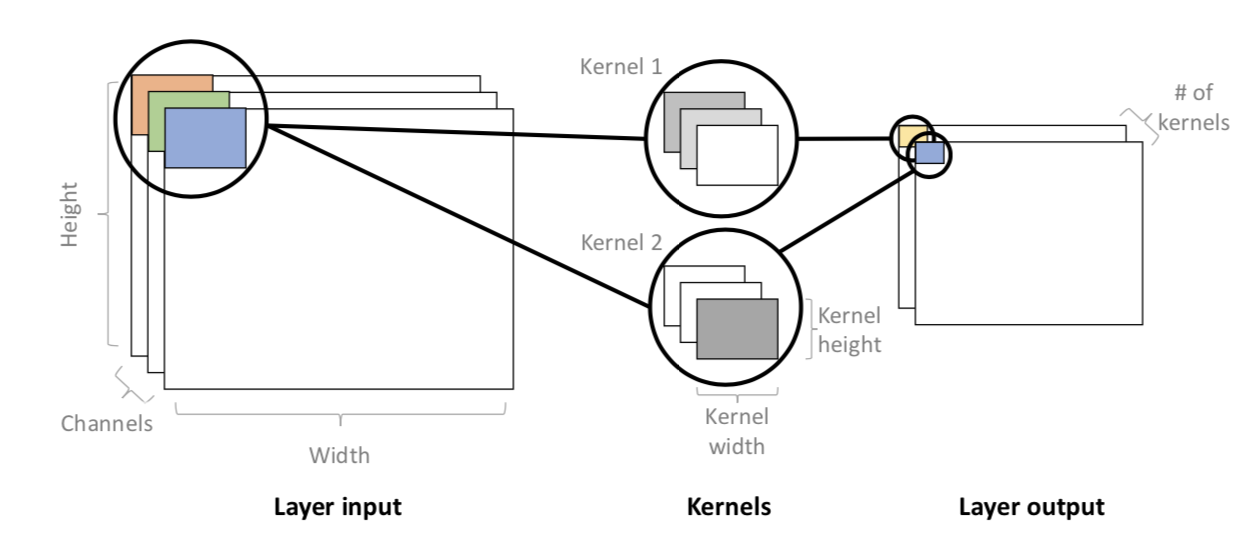
\includegraphics[width=0.95\textwidth]{math/cnn}
		\caption{A convolutional layer with two kernels that operate over different channels of a two-dimensional input. Figure from \cite{Gal2016UncertaintyThesis}.}
  	\label{fig:math_cnn}
\end{center}
\end{figure}

\subsection{Supervised Training}
Given a (convolutional) neural network with a set of parameters $\GenericParameters$ (where $\GenericParameters$ may include weight and bias parameters, $\Matrix{W}_\ell, \Matrix{b}_\ell$, as well as convolutional kernel parameters, $\Matrix{K}_{k\ell}$) we can use \textit{supervised training} to obtain an optimal parameter set $\GenericParameters^*$. Supervised training requires  set of training pairs $\{(\Vector{x}_1, \Vector{y}_1),...,(\Vector{x}_N, \Vector{y}_N) \}$ where $\Vector{x} \in \Real^{D_x}$ is an \textit{input} and $\Vector{y} \in \Real^{D_y}$ is a \textit{target} that corresponds to the desired output of our parametric model. To \textit{train} the network, we find the parameters which minimize a \textit{loss function} over this dataset,
\begin{equation}
\label{eq:math_nn_loss}
\GenericParameters^* = \ArgMin{\GenericParameters} \mathcal{L}\left(\{NN(\Vector{x}_i; \GenericParameters), \Vector{y}_i\right\}_{i=1}^N).
\end{equation}
For example, a common loss function for regression problems is \textit{mean squared error},
\begin{equation}
\GenericParameters^* = \ArgMin{\GenericParameters} \frac{1}{2N}\sum_{i=1}^N\Norm{NN(\Vector{x}_i; \GenericParameters) - \Vector{y}_i}_2^2.
\end{equation}.
In this dissertation, we will use supervised training in \Cref{ch:dpc,ch:sun-bcnn,ch:hydranet} and we will explore different forms of loss functions for geometric quantities that do not allow for a simple Euclidian norms. 
\subsection{Practical Considerations}
\label{section:math_dl_practical}
\subsubsection{Optimization}

To train a deep network---that is, to solve \Cref{eq:math_nn_loss} for optimal parameters---modern approaches rely on stochastic gradient descent (SGD) through back-propagation \citep{LeCun2015-qf}. SGD avoids the computationally prohibitive task of computing a gradient over an entire dataset by approximating the gradient using a randomly selecting subset of training data called a \textit{mini-batch}. In the majority of this dissertation, we rely on Adam, a modern SGD-based approach that also maintains an estimate of second-order curvature \citep{kingma_adam_2017}.

\subsubsection{Regularization}

In order to prevent \textit{overfitting} to a dataset (i.e., to obtain a model that generalizes to unseen data), the literature provides a number of methods. An important approach that is used in this dissertation is \textit{dropout} \citep{srivastava_dropout_2014}. Dropout stochastically `zeros-out' inputs of a particular layer with probability $p$, 

\begin{equation}
	\Vector{z}_{\ell+1} = \Vector{f}_\ell(\Vector{z}) = \Vector{\sigma}\left(\Matrix{W}_\ell\tilde{\Vector{z}}_\ell + \Vector{b}_\ell\right),
\end{equation}
where $\tilde{\Vector{z}}_\ell = \Vector{b} \circledcirc \Vector{z}_\ell$, $b_i \sim \text{Bernoulli}(p)$ and $\circledcirc$ refers to element-wise multiplication, also known as the Hadamard product.
The intuition behind dropout is that it effectively creates an ensemble of smaller-parameter networks that will generally be less prone to overfitting than a commensurately-sized monolithic network. Importantly, dropout has a fundamental connection variational inference, which we exploit in \Cref{ch:sun-bcnn}.
\subsubsection{Pooling and Spatial Invariance}
A common technique in convolutional neural networks is \textit{pooling} \citep{Goodfellow-et-al-2016}. Pooling is a non-parametric operation that summarizes the output of a kernel in a particular region. For example, \textit{max pooling} selects the maximum response of a kernel in demarcated regions of an input channel, thereby downsampling the resulting output. Pooling operations are designed to make convolution operations invariant to the spatial location of a particular kernel response. This is important in many classification tasks (e.g., a tree classifier should be invariant to the location of a particular leaf) but is a detriment to regression tasks where we would like to preserve spatial information. We explore building convolutional neural networks without pooling in \Cref{ch:dpc}.



 